% !TEX root = ../../../thesis.tex
The fabrication followed the method outlined in Section \ref{sec:method-sample-fabrication}. Due to a machine malfunction we deposited \qty{113}{\nano\meter} of \ce{Nb} instead of of \qty{90}{\nano\meter}\footnote{This was measured using an Atomic Force Microscope (AFM) by M. Westerdijk.}. The fine structures we made using the Focussed Ion Beam (FIB), can be seen in Figure \ref{fig:CP1.2H-SEM-images}.

\begin{figure}[ht]
	\begin{subfigure}[t]{0.3\textwidth}
		\centering
		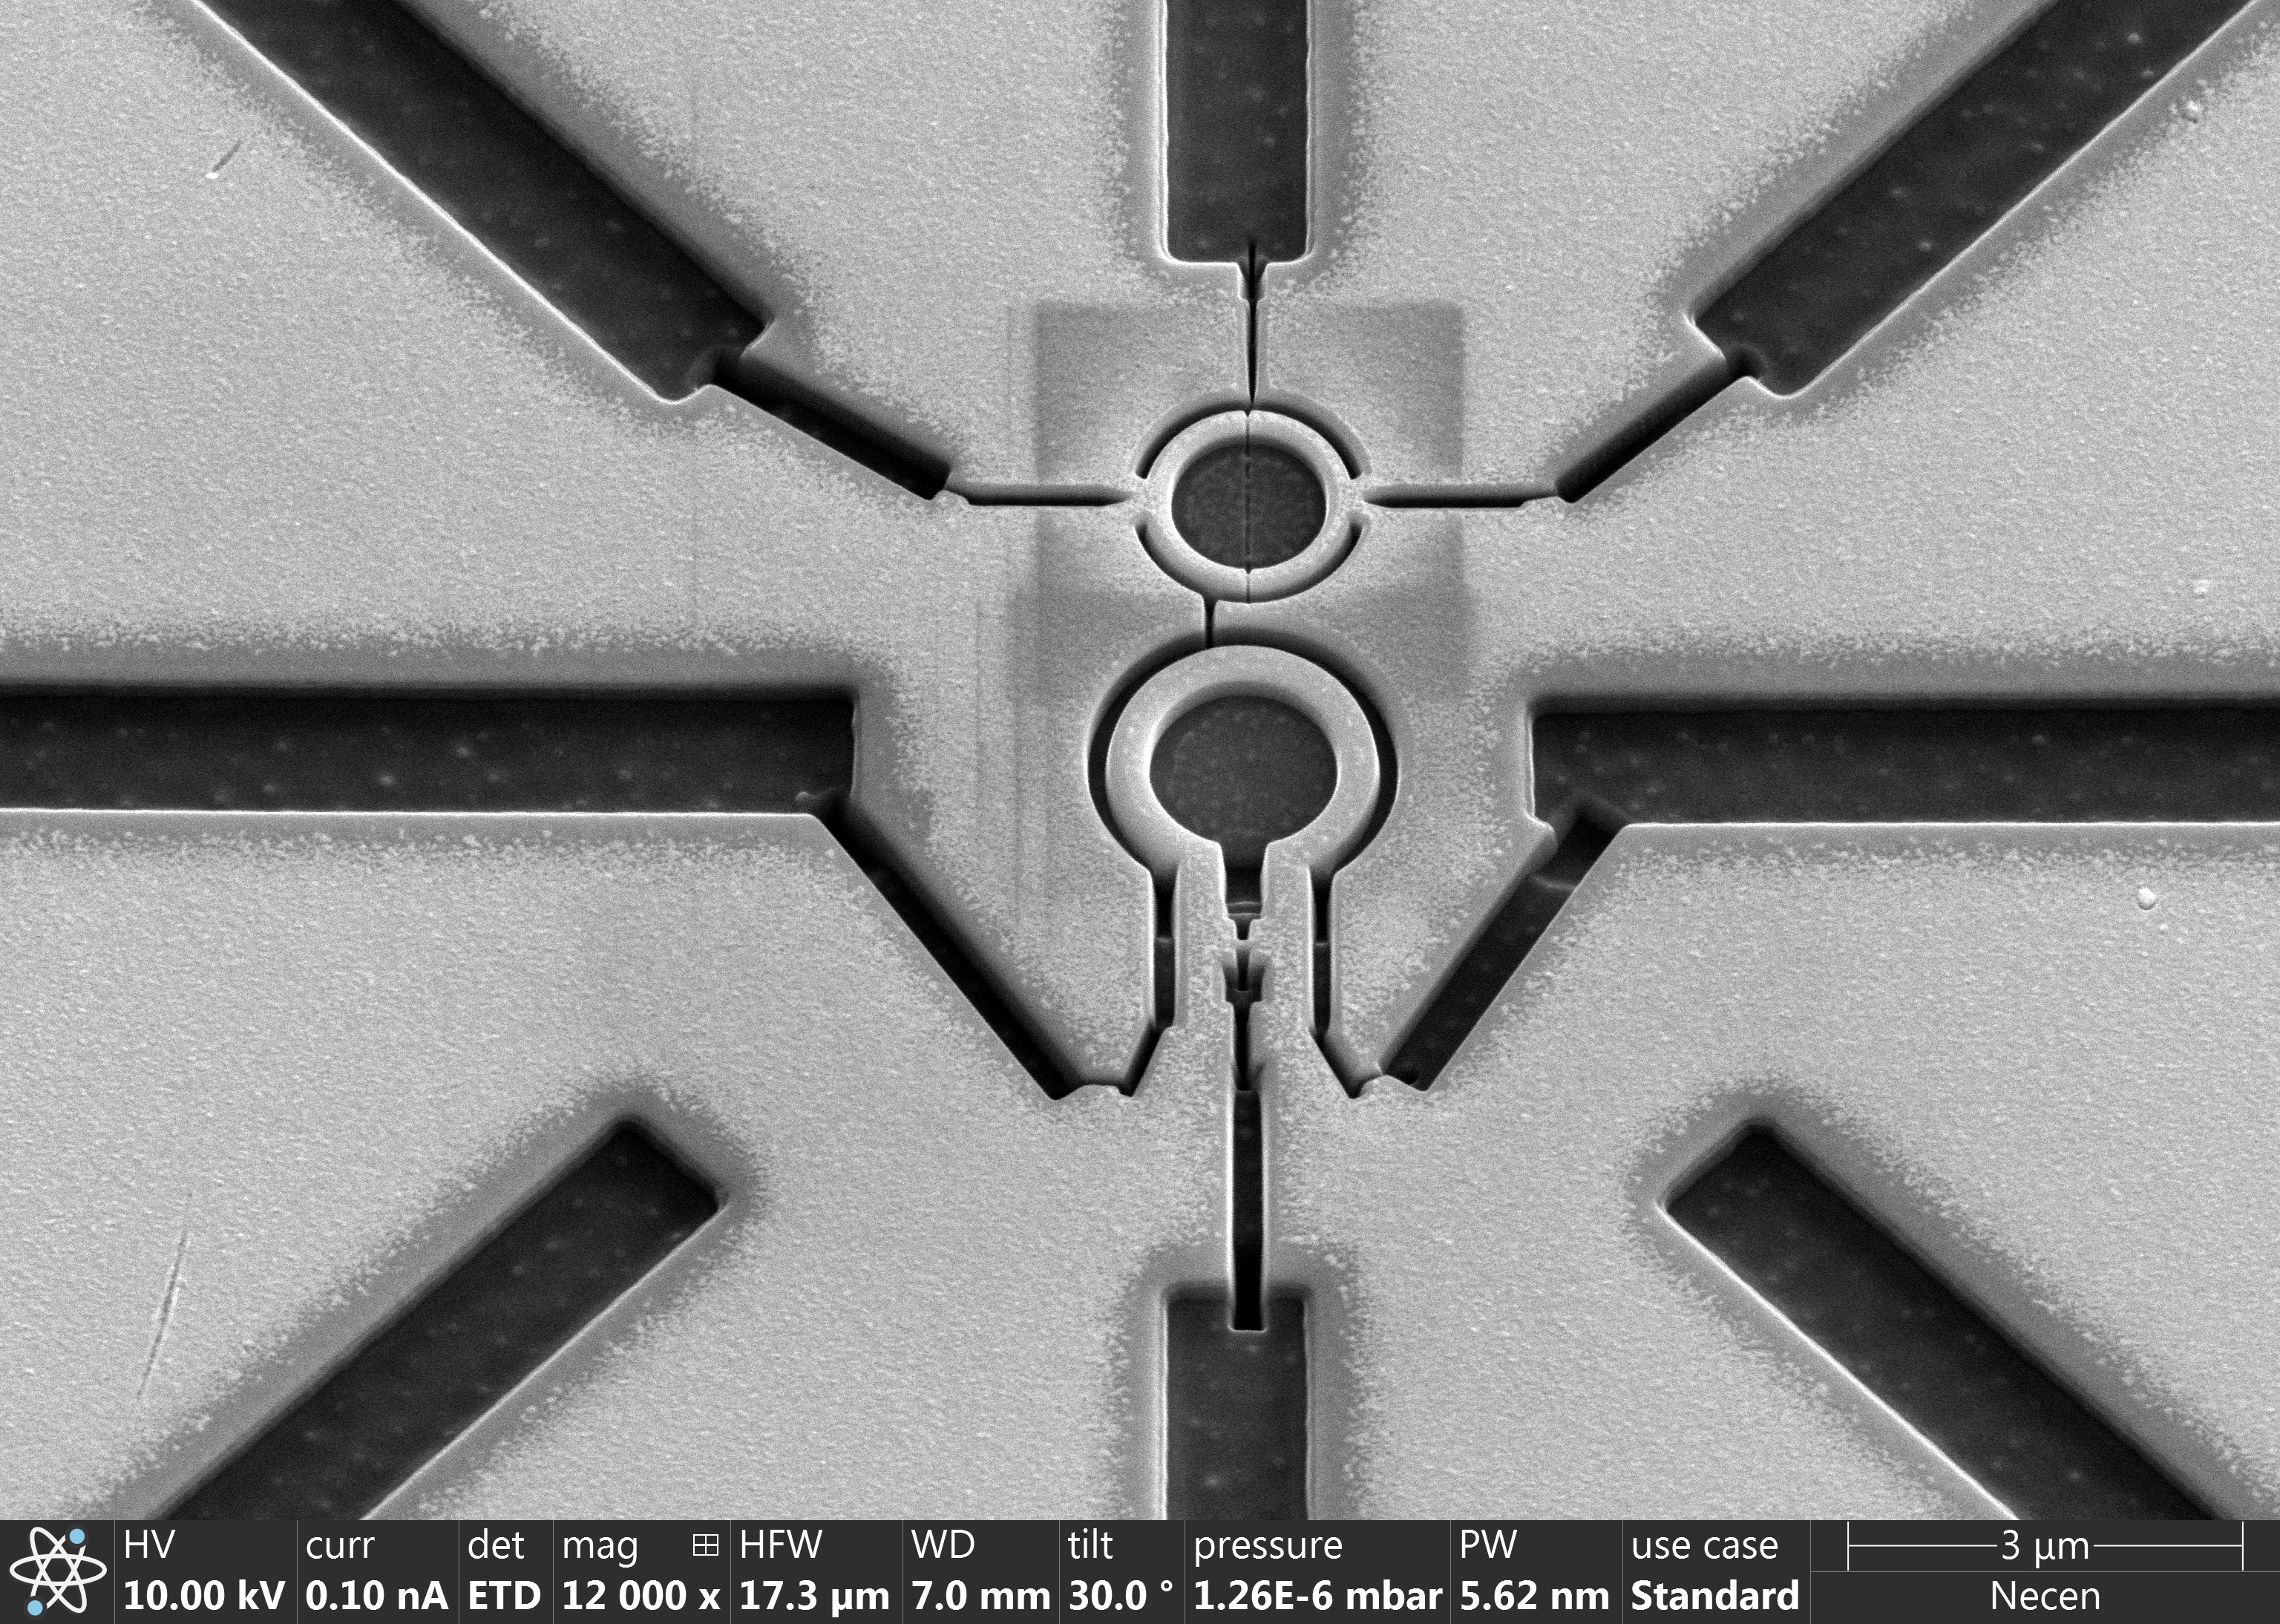
\includegraphics[width=\textwidth]{figures/samples/CP1/CP1.2H_SEM_overview.jpg}
		\subcaption{Overview of the fine structures. The thick leads go to \qty{300}{\micro\meter} by \qty{300}{\micro\meter} contact pads. On top we see the dc-SQUID and on the bottom the junction loop.}
	\end{subfigure}
	\hfill
	\begin{subfigure}[t]{0.3\textwidth}
		\centering
		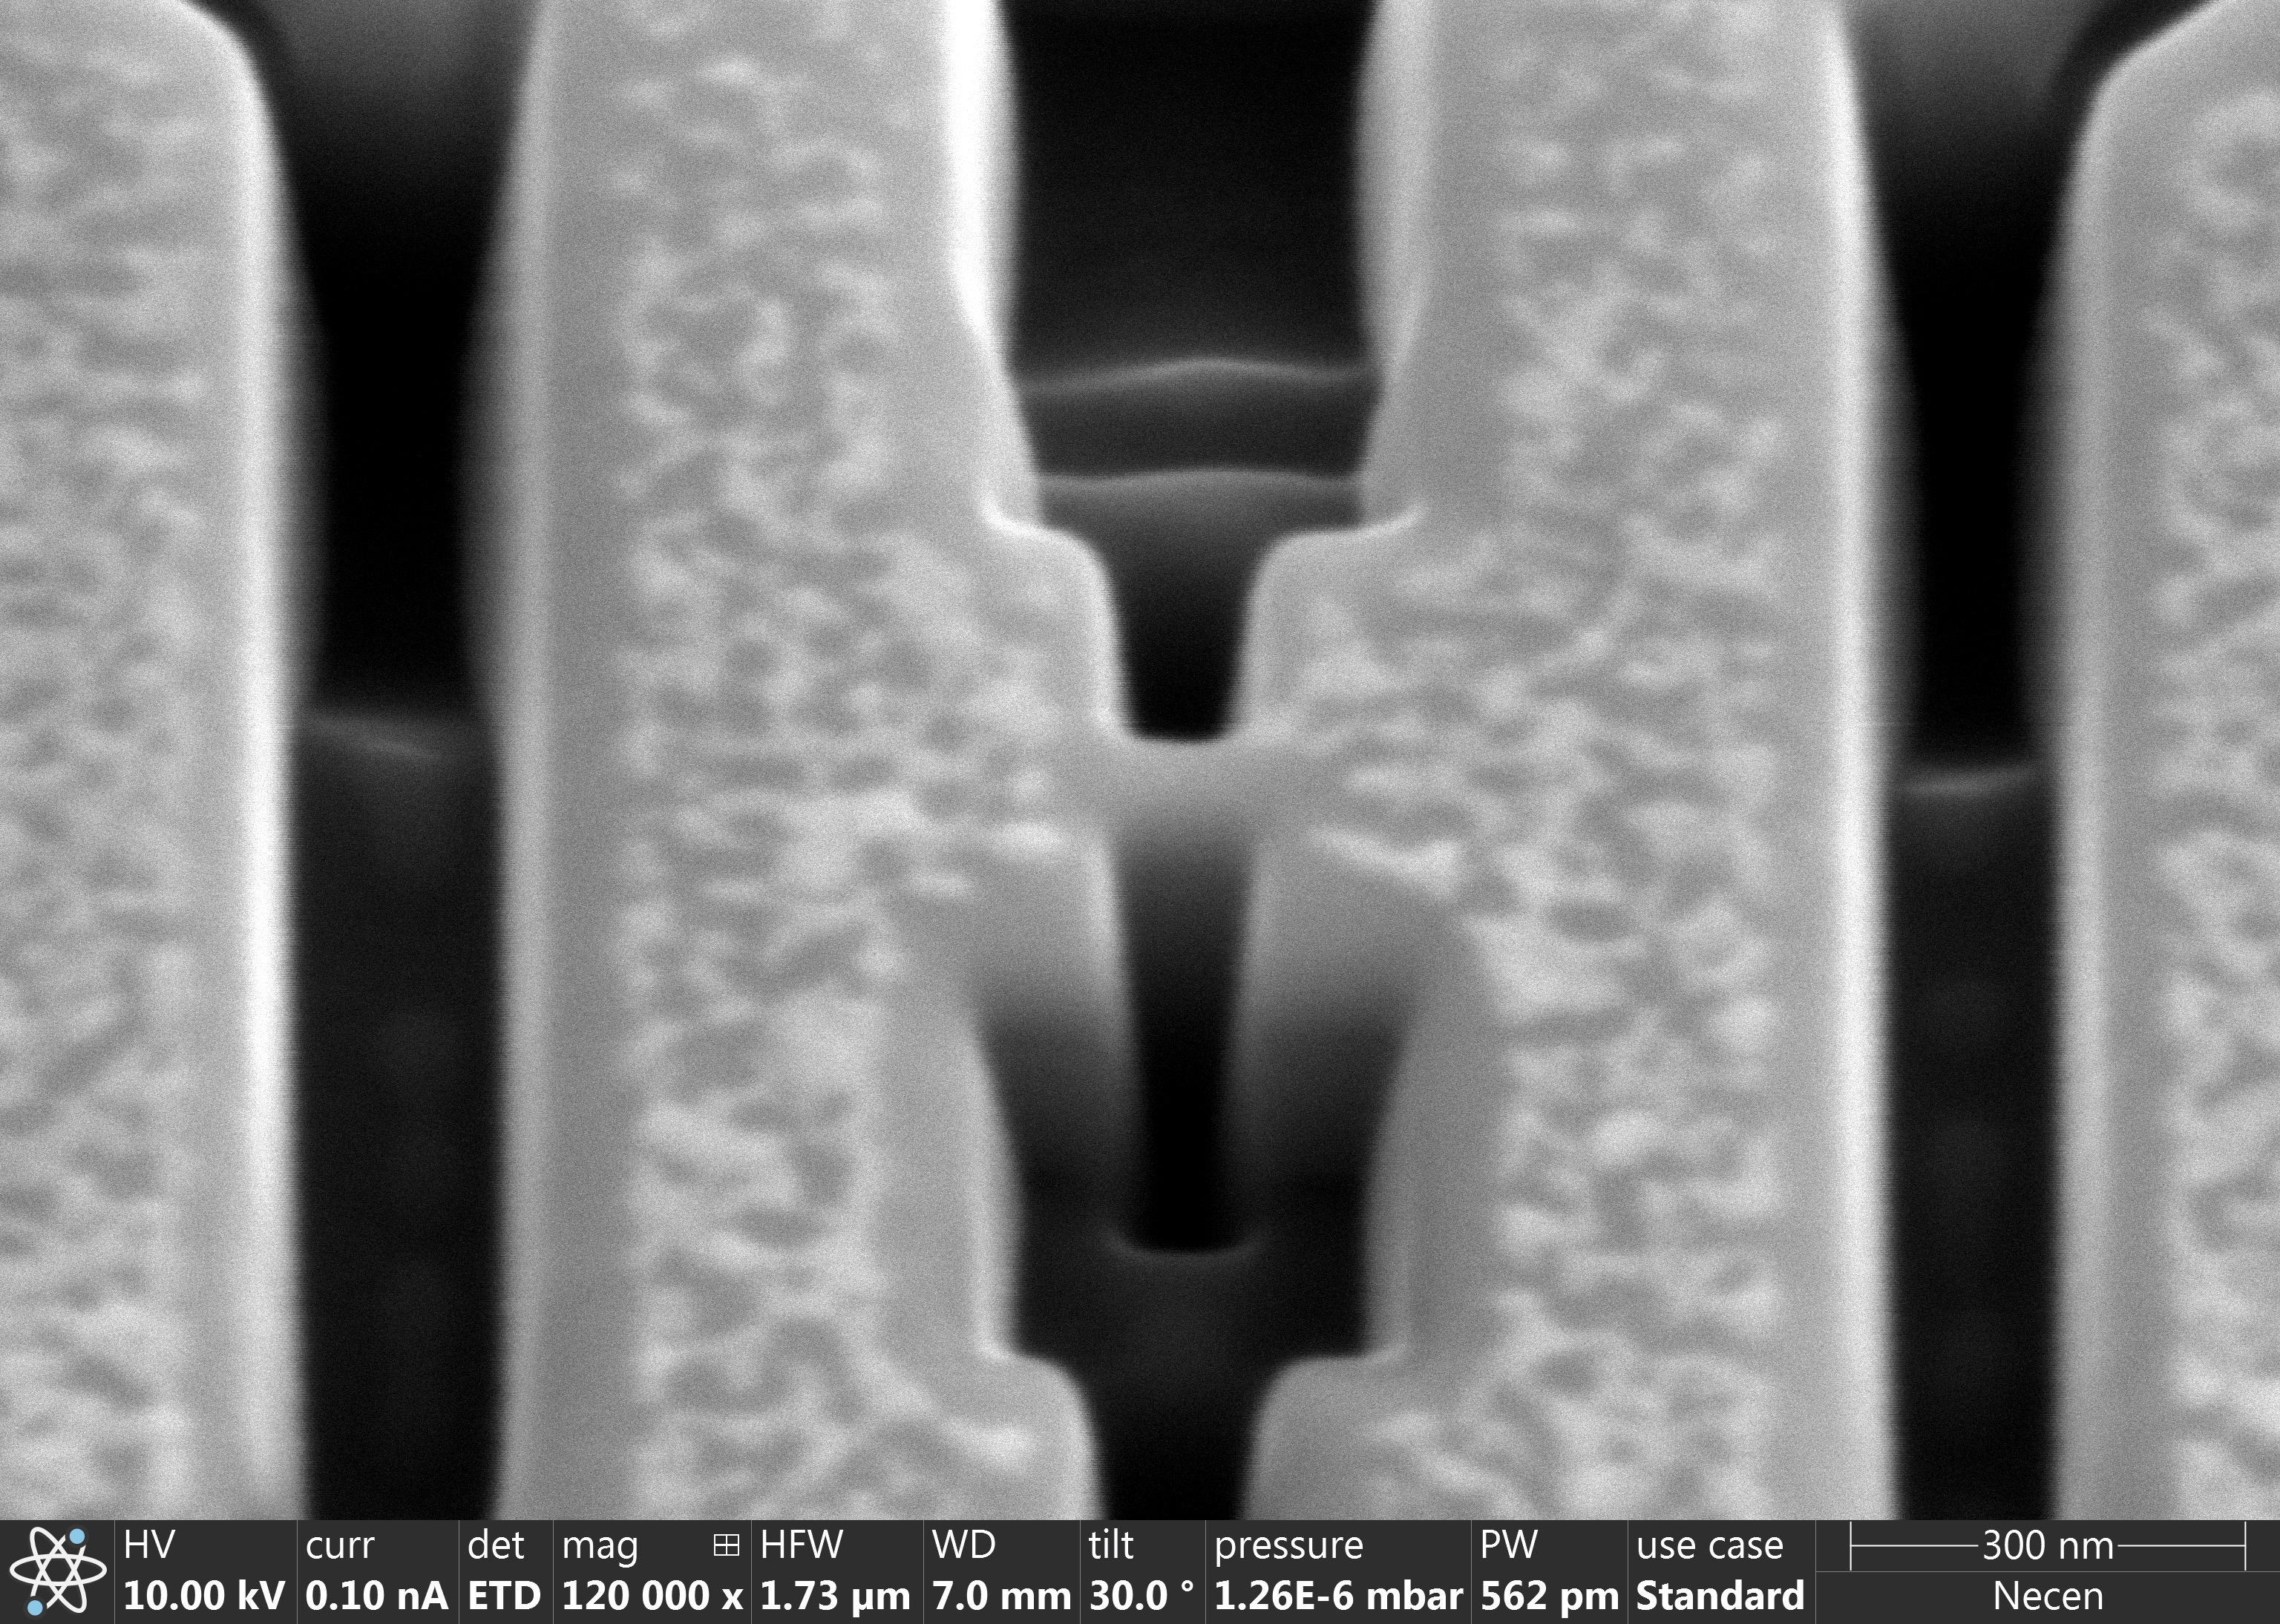
\includegraphics[width=\textwidth]{figures/samples/CP1/CP1.2H_SEM_junction.jpg}
		\subcaption{Zoomed in view of the junction, the size of the junction is \qty{100}{\nano\meter} by \qty{80}{\nano\meter}.}
	\end{subfigure}
	\hfill
	\begin{subfigure}[t]{0.3\textwidth}
		\centering
		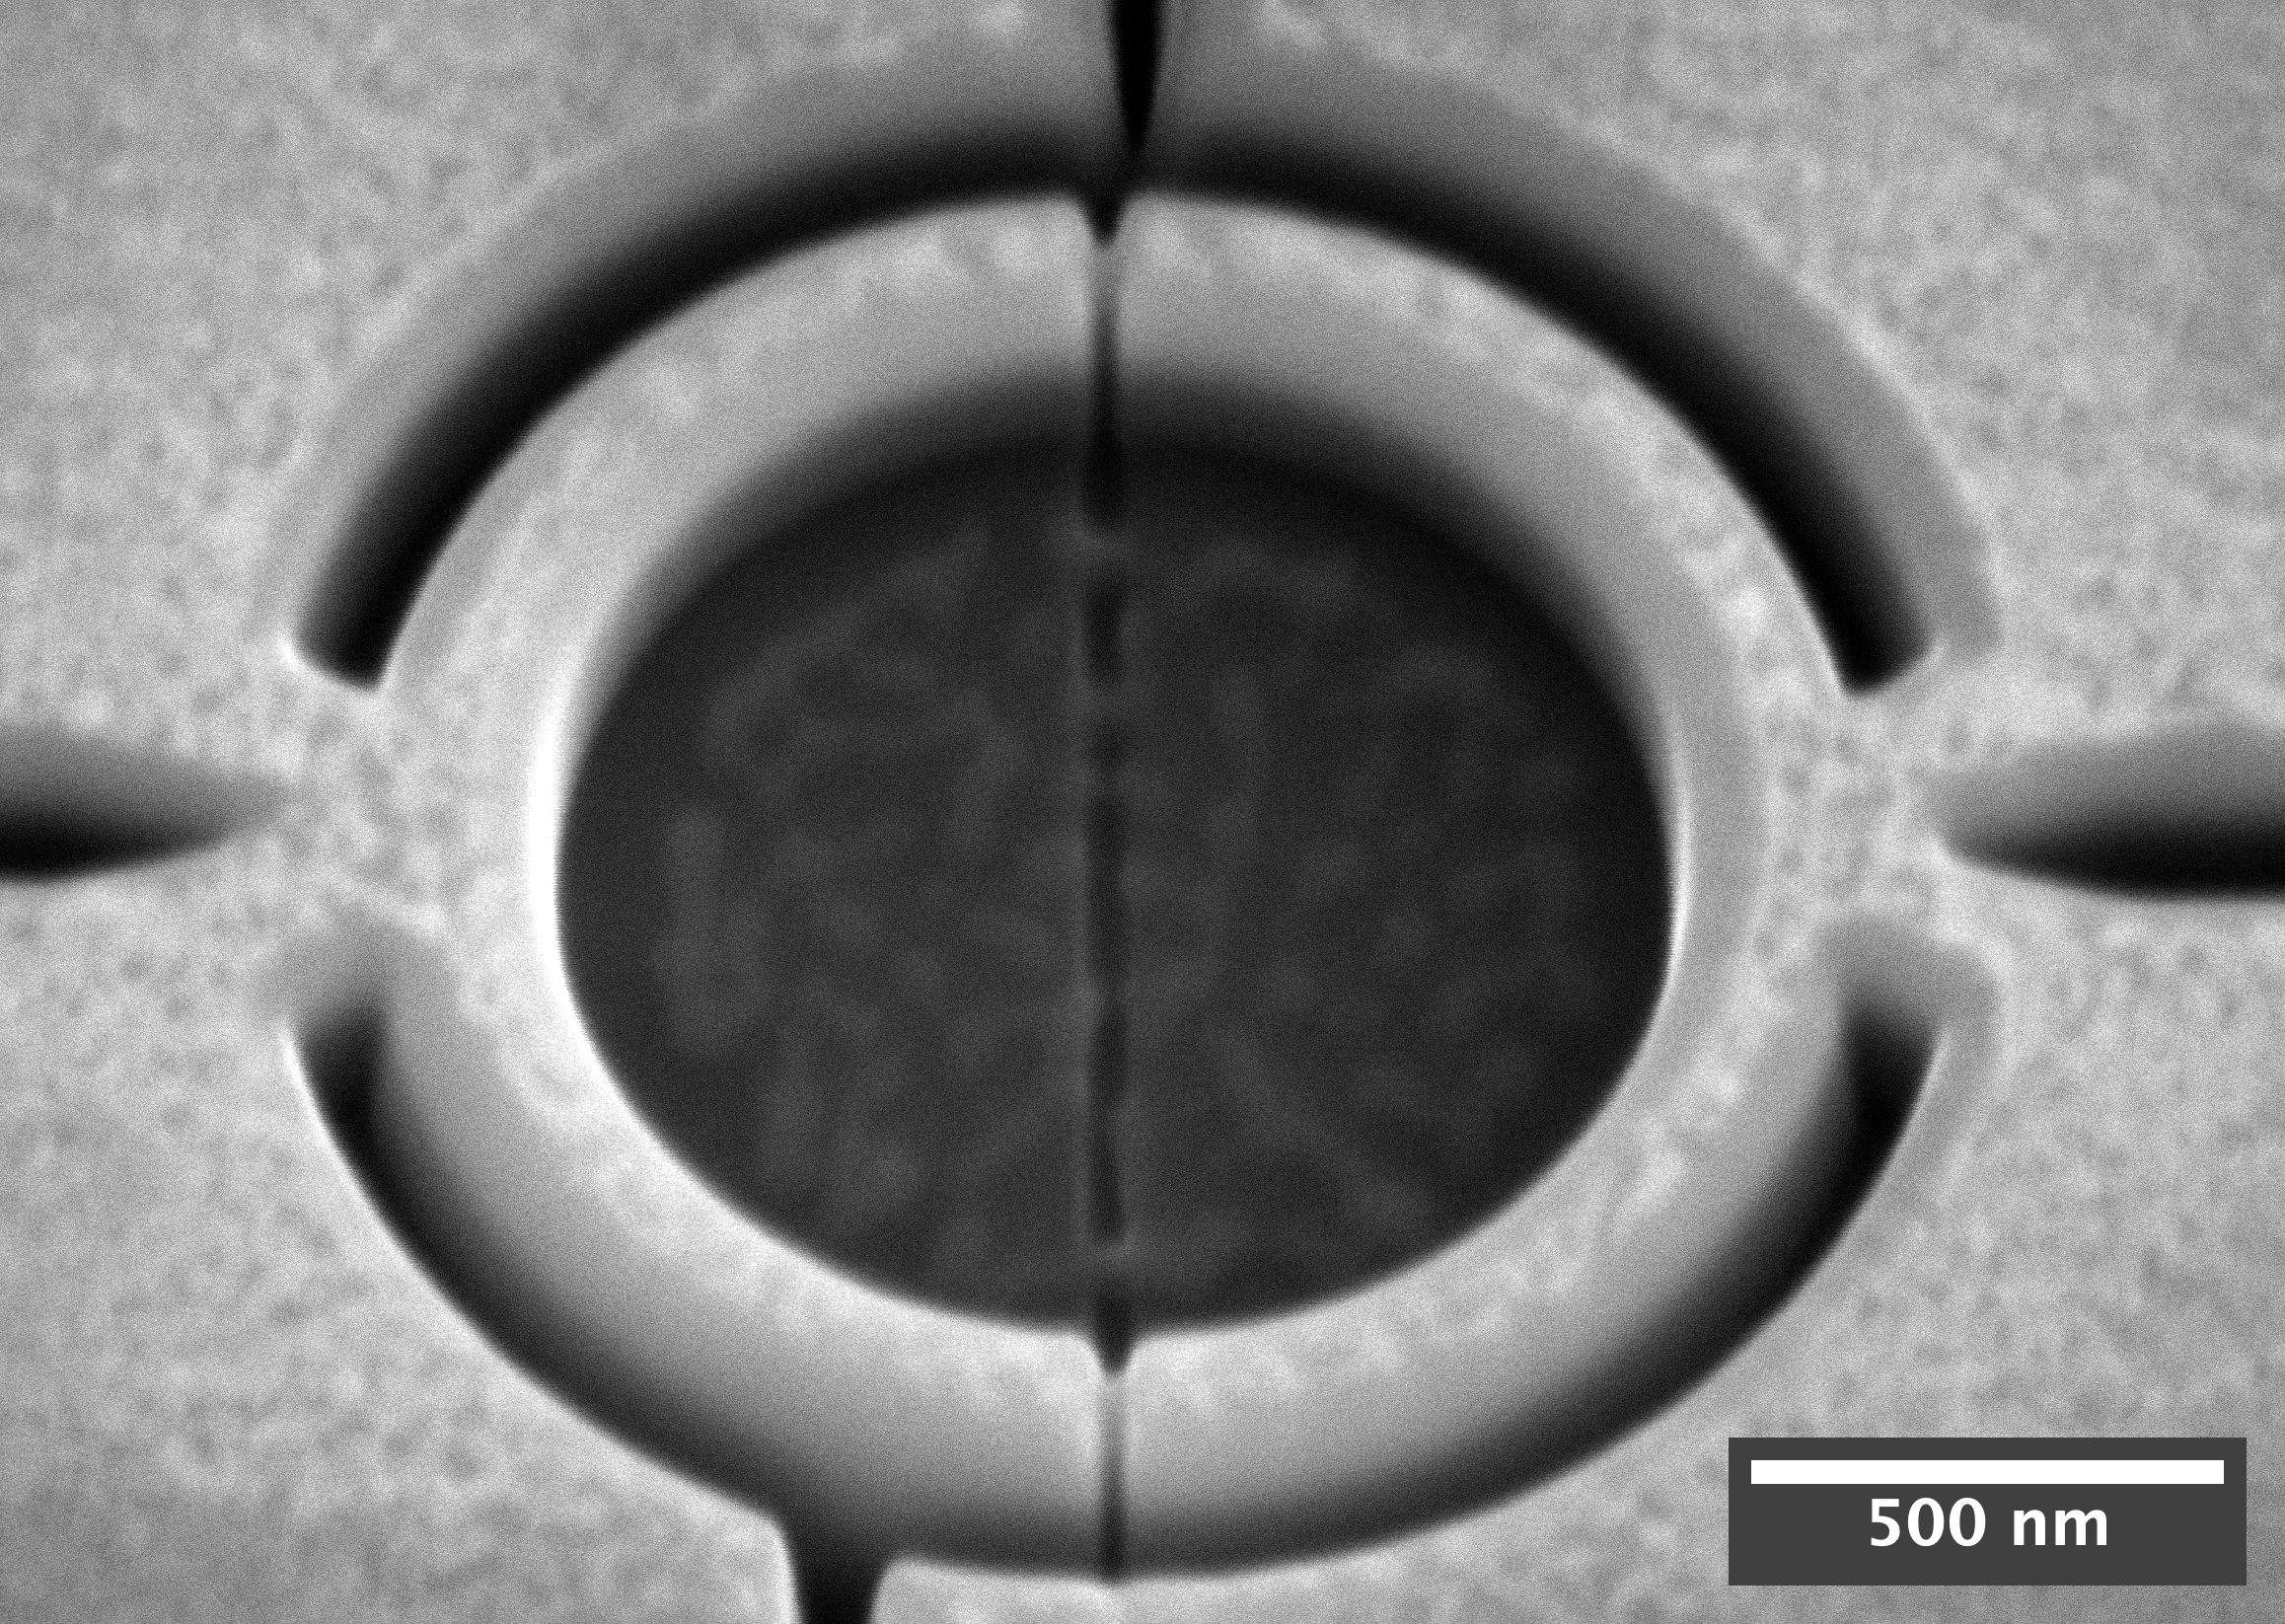
\includegraphics[width=\textwidth]{figures/samples/CP1/CP1.2H_SEM_SQUID.jpg}
		\subcaption{Zoomed in view of the dc-SQUID. The width of the junctions is \qty{19}{\nano\meter}.}
	\end{subfigure}

	\caption{Fine structures of sample CP1.2H after the FIB. See Table~\ref{tab:CP1.6H-geometries} for the exact geometries of the sample.}
	\label{fig:CP1.2H-SEM-images}
\end{figure}

\begin{table}
	\begin{subtable}{.5\linewidth}
		\centering
		\begin{tabular}{@{}lrr@{}}
			\toprule
			Parameter & Value \\ \midrule
			Junction loop $\diameter_{\text{outer}}$ & \qty{2.1}{\micro\meter} \\
			Junction loop $\diameter_{\text{inner}}$ & \qty{1.5}{\micro\meter} \\
			dc-SQUID $\diameter_{outer}$ & \qty{1.6}{\micro\meter} \\
			dc-SQUID $\diameter_{inner}$ & \qty{1.2}{\micro\meter} \\
			spacing & \qty{0.4}{\micro\meter} \\
			$d_{\ce{Nb}}$ & \qty{113}{\nano\meter} \\
			$d_{\ce{Au}}$ & \qty{7}{\nano\meter} \\
			\bottomrule
		\end{tabular}
    \end{subtable}
    \begin{subtable}{.5\linewidth}
    	\centering
    	\begin{tabular}{@{}lrr@{}}
    		\toprule
    		Parameter & Value \\ \midrule
    		$L_{l}$ & \qty{3.6}{\pico\henry} \\
			$L_{s}$ & \qty{3.1}{\pico\henry} \\
			$M$ & \qty{-0.1}{\pico\henry} \\
			$\delta$ & \num{0.00006} \\
			$\kappa$ & \num{-0.016} \\
    		\bottomrule
    	\end{tabular}
    \end{subtable}
    \caption{The \textbf{left} table provides an overview of the geometries of CP1.6H as determined by SEM imaging and sputtering rates. The \textbf{right} table gives an overview of parameters found using a simulation based on the geometries. The geometries of the dc-SQUID are based on earlier work by \citeauthor{rogSQUIDontipMagneticMicroscopy2022} \citeyear{rogSQUIDontipMagneticMicroscopy2022}.}
    \label{tab:CP1.6H-geometries}
\end{table}